\documentclass[11pt]{article}
\usepackage[margin=0.85in]{geometry}
\usepackage{amsmath,amssymb,graphicx,hyperref}
\setlength{\parindent}{0pt}\setlength{\parskip}{6pt}
\setlength{\emergencystretch}{3em}
\begin{document}
{\Large Actual target-branch radical is the witness line}\\
November 13, 2026. Symbolic transfer; unsigned evidence [pcc:unverified].

\textbf{Objects and guards.} Over any field, let $F,H$ be monic and
$0<\deg H$, $\deg H+1<\deg F$, $UF+VfH=1$. Define
\[
 \mu(P)=[X^{\deg F-1}](PV\bmod F),\qquad
 \mathcal B((A,B),(Q,T))=\mu(AQ-fBT).
\]
Both polynomial pairs have degree caps $(\deg F,\deg H)$. The actual branch is
$\ell(A,B)=A(q)-yB(q)$. Assume $F(q)\ne0$, $\alpha\ne0$ and
$\ell(\alpha F,\beta H)=0$. For every admissible branch pair $(A,B)$:
\[
 \mathcal B((A,B),(Q,T))=0\ \text{for all admissible branch tests}
 \quad\Longleftrightarrow\quad
 (A,B)=t(\alpha F,\beta H).
\]
The witness direction is nonzero. If its supplied actual norm is $cG$, the
norm on that line is $t^2cG$. No literal matrix rank is assumed.

\textbf{Constructive proof.} Set $s=(Q(q)-yT(q))/F(q)$ and $Q'=Q-sF$.
Then $(Q',T)$ is on the branch and retains its degree caps. The exact identity
\[
 A(Q-sF)-fBT=(AQ-fBT)-F(sA)
\]
and annihilation of every modulus multiple give the same actual pairing.
Branch tests therefore detect exactly the full radical. The existing block
radical theorem gives $(A,B)=(cF,dH)$. The two branch equations imply
$\alpha d=\beta c$ after cancelling $F(q)$, and $t=c/\alpha$ gives the line.
There is no division by $2$, $y$, $H(q)$ or $\beta$.

\begin{center}
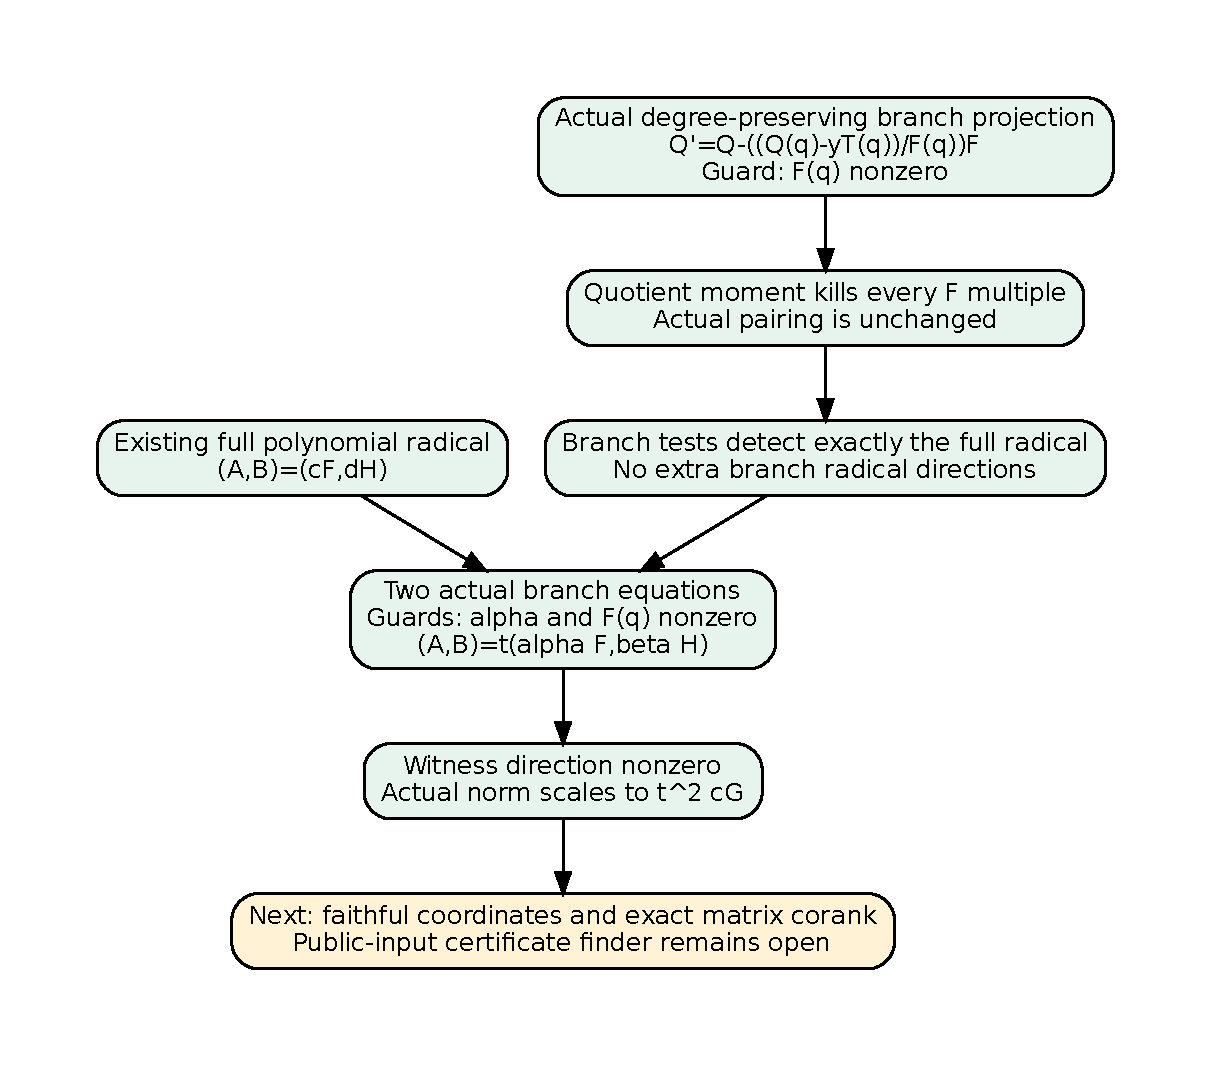
\includegraphics[width=0.98\linewidth,height=0.37\textheight,keepaspectratio]{branch.pdf}
\end{center}

\newpage
{\Large Formal evidence and next transfer}

\textbf{Formal map.} Frozen source \path{38b91e915},
\path{NormBranchRadical.lean}, has nine declarations:
Its nine declarations cover the universal projection identity, actual moment
annihilation, branch projection and pairing preservation, restricted versus full
tests, scalar elimination, the witness-line radical, witness nonzeroness and
actual norm scaling. Exact hypotheses and unsigned
producer PCC bindings are linked from the Markdown report.

\textbf{Checks.} Target build004 completes3148 jobs with pinned Lean4.35.0,
CryptoLean148f5dc and Mathlibcfc55fc. The full tracked-source gate and fresh
import-inclusive replay have attributable completion receipts. Only standard
foundations are admitted; no signed PCC verdict is claimed. Draft001 failed
on opaque moment unfolding and a division implication. Draft002 uses the
exported momentApply and a direct equality; builds003/004 add the universal
identity, nonzero witness and norm scaling. Failed logs are retained.

Native record \path{IDC1h75cd0c4ee7db5e5d} checks only the universal CommRing
projection identity at32 statement-derived plus32 extra-stream points through
the unchanged maintained checker. It does not execute Lean or prove branch
guards, radical dimension or search cost. Its22 inherited tests pass.

\textbf{Certificate scope.} The supplied witness and Bezout data determine
the quotient functional. This result gives no public-input method for finding
them. The annotated nonscalar-origin/jet-completion proposal has a separate,
unproved reachability obligation; this functional is not shown to be reachable
as $W_{\mathrm{base}}+C(T)H(T)$. The lower norm polynomial named $H$ here does
not construct that jet correction. Constant-$H$ and degree-drop charts remain
separate.

\textbf{Next proof obligations.} Transfer the actual product-basis coordinates
faithfully to the two bounded polynomial spaces, including degree bounds and
injectivity. Expand the matrix bilinear expression for arbitrary vectors, then
use a genuine basis of the branch kernel. Transfer the single nonzero radical
line to exact matrix corank, a nonzero adjugate and every stationarity guard
required by recovery. The finder and its uniform bit cost remain additional
obligations.

\textbf{Sources.} Prior local block-radical, branch-test and moment theorems;
source-linked matrix/functional continuation plans; pinned Mathlib polynomial
natDegree bounds. Primary summation-polynomial context remains Galbraith15.8.1--2,
source-pinned in the cost audit. This elementary projection has no priority claim.
KB MCP/wrapper and conductor unavailable; bounded fallback only.

\textbf{Resources.} Local proof and expression-correctness checks only. No
Python mathematical research, new paid job or timing/scaling campaign. Monthly
isolab budget remains exhausted. No benchmark, leaderboard or ecdb result;
canonical scoreboards and historical measured figures remain unchanged.
Editable DOT/SVG, source-linked report and exact receipts accompany this PDF.
\end{document}
